\subsection{Unsaturated Model Parameters ($\theta_{\nox}$) \label{sec::unsat_est}}

With the saturated segments excluded, the remaining data satisfies the unsaturated
dynamics~(\ref{eqn::eta_bar_dynamics}). These data can now be used for least-squares estimation of $\theta_{\nox}$.

\subsubsection{Regression Form}

The compact form $\bar\eta_F(k{+}1) = \bar\eta_F(k) + \phi_{\nox}^T(k)\,\theta_{\nox}$~(\ref{eqn::eta_compact})
rearranges into a standard linear regression by moving $\bar\eta_F(k)$ to the left:
\begin{align}
    y_{\nox}(k) &= \phi_{\nox}^T(k)\,\theta_{\nox}
    \label{eqn::regression_form}
\end{align}
where $y_{\nox}(k) = \bar\eta_F(k{+}1) - \bar\eta_F(k)$. The regressor $\phi_{\nox}(k)$ depends only on measured
quantities and is constructed to avoid unnecessary multiplication and division of the same signals, which would amplify
noise.

$\theta_{\nox}$ is estimated by least squares on the unsaturated segments identified
in~\S\ref{sec::segment_id}. Under Gaussian model structure error, least squares is the maximum likelihood
estimate. These are the same parameters that appear in the guard
condition~(\ref{eqn::guard_condition}), so once estimated, the guard is fully determined.

\subsubsection{Estimation Results}

With both $\hat\theta_{\sat}$ and $\hat\theta_{\nox}$, the full switched model~(\ref{eqn::switched_model}) is simulated
from initial conditions and inputs ($u_1, u_2, F, T$) alone on the training data. The goodness of fit is measured by:
\begin{align}
    \%\text{fit} = 100 \times \lr{1 - \frac{\norm{Y - \hat Y}}{\norm{Y - \text{mean}(Y)}}}
\end{align}

\begin{table}[!ht]
    \centering
    \caption{Goodness of fit on training data}
    \label{tab::results}
    \begin{tabular}{l l c c}
        \hline \hline
        Age & Test & Switched model & CSTR baseline \\
        \hline \hline
        Degreened & RMC      & 71.9\% & 20.0\% \\
        Aged      & RMC      & 69.9\% & 27.7\% \\ \hline
        Degreened & hot-FTP  & 61.9\% & 7.1\%  \\
        Aged      & hot-FTP  & 63.5\% & 7.4\%  \\ \hline
        Degreened & cold-FTP & 52.9\% & 23.2\% \\
        Aged      & cold-FTP & 60.3\% & 23.2\% \\
        \hline \hline
    \end{tabular}
\end{table}

\begin{figure}[!ht]
    \begin{minipage}{0.24\textwidth}
        \centering
        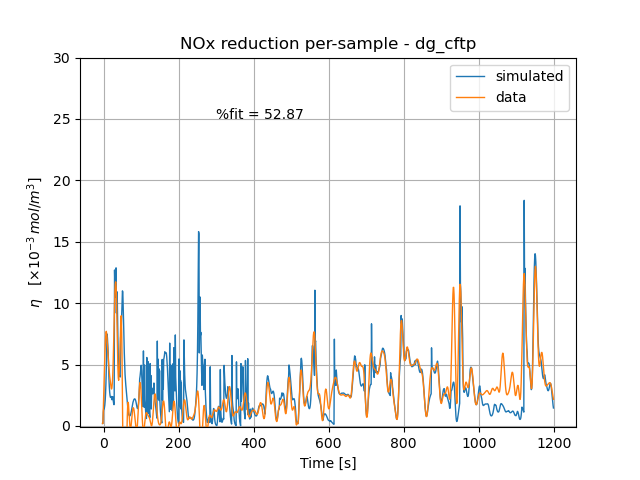
\includegraphics[width=\textwidth]{./figs/3-sysID/eta_sim_dg_cftp.png}
    \end{minipage}
    \begin{minipage}{0.24\textwidth}
        \centering
        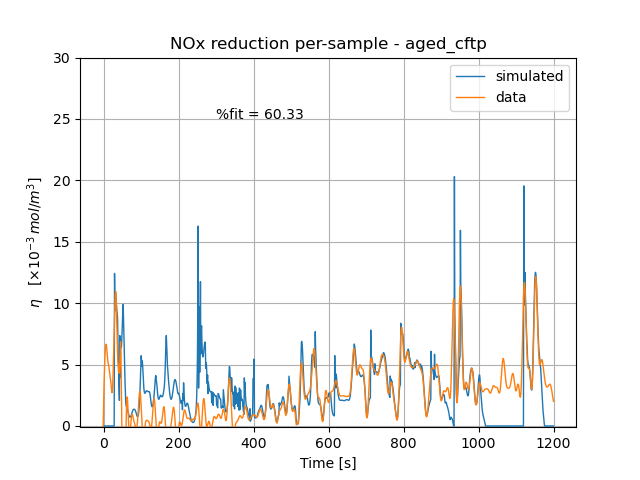
\includegraphics[width=\textwidth]{./figs/3-sysID/eta_sim_aged_cftp.png}
    \end{minipage}
    \caption{Simulation: cold-FTP}
    \label{fig::eta_sim_cftp}
\end{figure}

\begin{figure}[!ht]
    \begin{minipage}{0.24\textwidth}
        \centering
        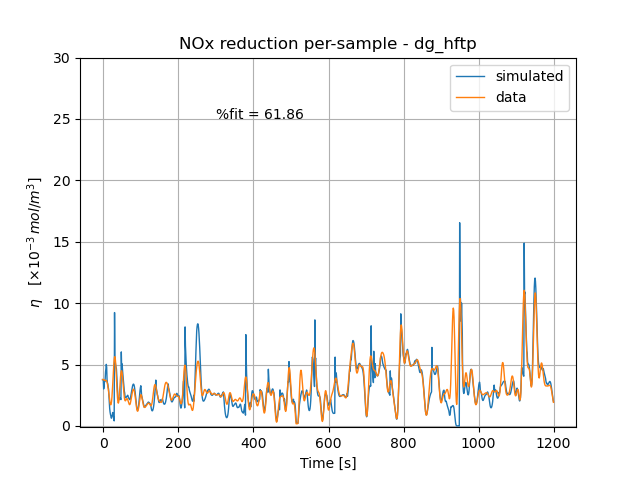
\includegraphics[width=\textwidth]{./figs/3-sysID/eta_sim_dg_hftp.png}
    \end{minipage}
    \begin{minipage}{0.24\textwidth}
        \centering
        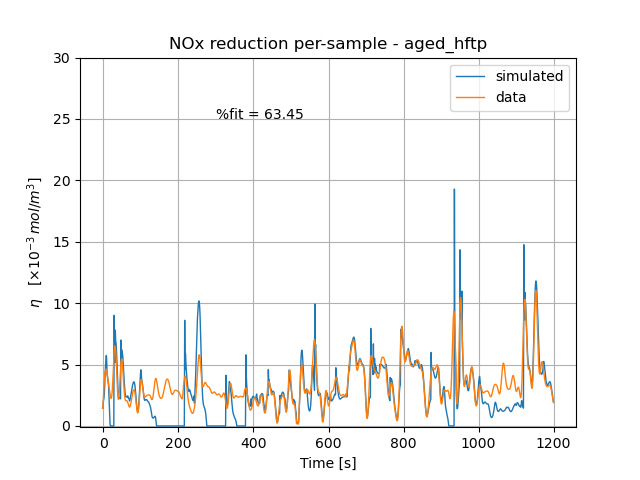
\includegraphics[width=\textwidth]{./figs/3-sysID/eta_sim_aged_hftp.png}
    \end{minipage}
    \caption{Simulation: hot-FTP}
    \label{fig::eta_sim_hftp}
\end{figure}

\begin{figure}[!ht]
    \begin{minipage}{0.24\textwidth}
        \centering
        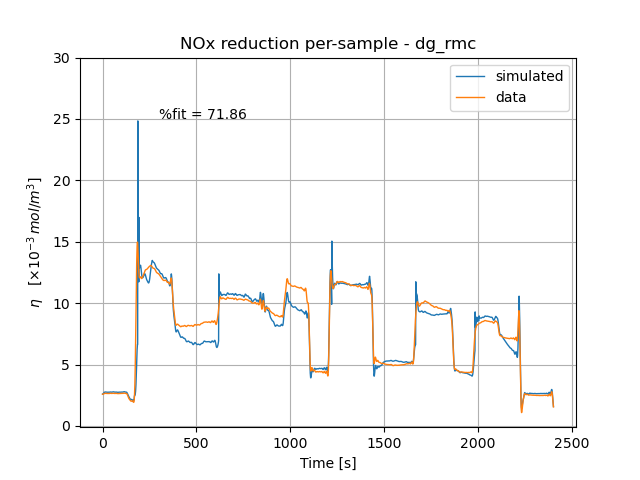
\includegraphics[width=\textwidth]{./figs/3-sysID/eta_sim_dg_rmc.png}
    \end{minipage}
    \begin{minipage}{0.24\textwidth}
        \centering
        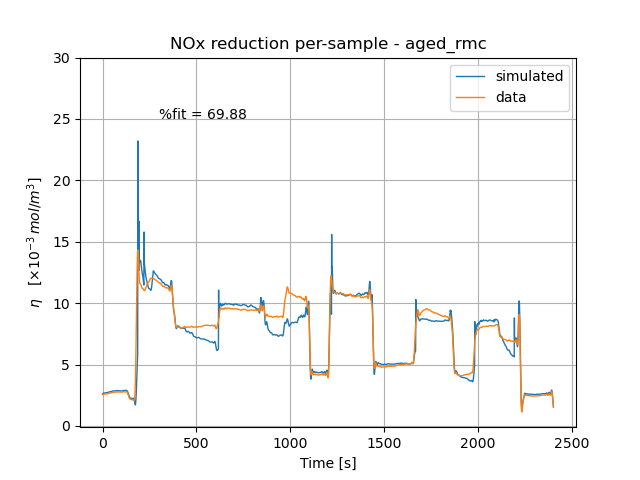
\includegraphics[width=\textwidth]{./figs/3-sysID/eta_sim_aged_rmc.png}
    \end{minipage}
    \caption{Simulation: RMC}
    \label{fig::eta_sim_rmc}
\end{figure}
